\documentclass[11pt,a4paper]{report}

\usepackage[polish]{babel}
\usepackage[utf8x]{inputenc}
\usepackage{polski}
%\usepackage[T1]{fontenc}
\frenchspacing
\usepackage{indentfirst}
\usepackage{amsthm}
\usepackage{amsmath}
\usepackage{algorithmic}
\usepackage{algorithm}
\usepackage{program}
\usepackage{programs}
\usepackage{array}
\usepackage{multirow}
\usepackage{graphicx}
\usepackage{listings}
\usepackage{listing}
\usepackage{float}
\pagenumbering{arabic}

\graphicspath{{img/}}

\begin{document}
\tableofcontents

\chapter{Preprocessing}

W aplikacji znajdują się trzy różne preprocessingi zebranych danych. Pierwsze dwa służą szybszemu wyliczaniu macierzy używanych przy algorytmach Adapted Pagerank i Social Pagerank. Algorytmy te przy każdym przebiegu korzystają z tych samych macierzy, obliczanie ich przy każdej iteracji wymagałoby dużego nakładu czasu. Trzeci preprocessing jest dla danych używanych są przy wyświetlaniu dla użytkownika wyników wyszukiwań.

\section{Tworzenie macierzy}

Dane dla algorytmów wyliczane są w dwóch częściach. Na początku wyliczane są dane w bazie danych i zapisywane w pomocniczych tabelach. Następnie zapisywane są one do do struktury i serializowane w oddzielnych plikach. Dane ze zserializowanych plików używane są później do tworzenia macierzy.

\subsection{Preprocessing w bazie danych}

W bazie danych wyliczone zostają informacje potrzebne do późniejszego utworzenia macierzy. Informacje te zostaną zapisane w tabeli USERTAGDOC w polu how\_much i w tabelach TAG\_USR i TAG\_DOC. Wyliczenie tych informacji pozwoli później na szybszy dostęp do nich.

Czas wykonania preprocessingu w bazie danych jest różny. Jak widać w tabeli poniżej (\ref{tab:czas_tabele}) najwięcej czasu trwało tworzenie tabeli TAG\_USR i powstało w niej najwięcej nowych rekordów. Prawdopodobnie jest to spowodowane tym, że użytkownicy używają różnych tagów przy oznaczaniu różnych dokumentów. Z drugiej strony, dokumenty, mimo ze opisywane są przez różnych użytkowników, oznaczone są najczęściej podobnymi tagami.

\begin{center}
\begin{table}
  
    \begin{tabular}{ | c | p{3cm}| p{3cm} | }
    \hline
    Tabela & czas wykonania polecenia & ilość powstałych rekordów  \\ 
    \hline
    TAG\_USR & 22h 34min 4s & 26,938,914   \\ 
    \hline
    TAG\_DOC & 3h 13min 23s  &  14,563,924\\ 
    \hline
    USERTAGDOC & 1h 34min 17s  & $14563924$  \\ 
    \hline
    \end{tabular}
     \caption{Czas wykonania wypełnienia odpowiednich tabel w bazie danych}
    \label{tab:czas_tabele}
   
\end{table}
\end{center}

Poniżej znajdują się listingi zapytań SQL updatujące tabele USRTAGDOC \ref{sql_usrtagdoc} i wypełniający tabele TAG\_USR (\ref{sql_tag_doc}) i TAG\_DOC (\ref{sql_tag_usr}). 


\lstset{language=SQL}   
\begin{lstlisting}[frame=lines, caption={Skrypt dodający dane do tabeli tag\_doc}, label={sql_tag_doc}]
insert into tag_doc (tag_id, doc_id, how_much)
select tag.id, utd.doc_id, 1
from
tag,
usertagdoc_tag as utd_t,
usertagdoc as utd
where
utd_t.usertagdoc_id = utd.id and
utd_t.tags_id = tag.id
on duplicate key update how_much=how_much+1;
\end{lstlisting}

\begin{lstlisting}[frame=lines, caption={Skrypt dodający dane do tabeli tag\_usr}, label={sql_tag_usr}]]
insert into tag_usr (tag_id, user_id, how_much)
select tag.id, utd.user_id, 1
from
tag,
usertagdoc_tag as utd_t,
usertagdoc as utd
where
utd_t.usertagdoc_id = utd.id and
utd_t.tags_id = tag.id
on duplicate key update how_much=how_much+1;
\end{lstlisting}

\begin{lstlisting}[frame=lines, caption={Skrypt updatujący pole how\_much w tabeli usertagdoc}, label={sql_usrtagdoc}] ]
update usertagdoc utd
set how_much = (select count(distinct tags.tags_id)
from usertagdoc_tag tags
where utd.id = tags.usertagdoc_id);
\end{lstlisting}


\subsection{Preprocessing: zapis do plików}
Zapis do plików mógłby być połączony z preprocessingiem w bazie danych. Powodów na rozdzielenie tego procesu jest kilka. Głównym powodem jest czas pobierania danych z bazy danych. O ile posiadamy wszystkie informacje w bazie danych już wyliczone nie możemy pobrać ich wszystkich jednocześnie. Zajmowałyby za dużo miejsca w pamięci. Musimy pobierać dane z bazy danych częściowo, w podzielone na fragmenty zależne od tworzonej macerzy i odpowiednio posortowane. Właśnie sortowanie wyników jest najbardziej czasochłonną częścią procesu.

Kolejnym powodem oddzielenia było to, że po stworzeniu plików algorytmy SociaPagerak i Adapted Pagerank są niezależne od bazy danych. W czasie ich działania możliwe jest zmieniane i odświeżanie danych w tabelach TAG\_USR i TAG\_DOC. 

Czas tworzenia plików jest zdecydowanie krótszy od operacji na bazie danych i wynosi około 6h. Samo tworzenie plików może zostać zrównoleglone w zależności od tabeli z której pobierane są informację. Zrównoleglenie powinno zdecydowanie przyśpieszyć czas tworzenia plików. 

Ilość danych w wierszy macierzy zapisanych w pliku jest konfigurowalna i zależna od przydzielonej pamięci aplikacji. Pamięć nie jest problem w czasie tworzenia plików, ale w czasie przebiegu interacji algorytmów. Tworzona macierz zajmuje dużo miejsca w pamięci, dlatego tworzone struktury które będą odserializowane z plików i przechowywane w pamięci muszą zmieścić się w ograniczonej pamięci z fragmentem macierzy.


Dane pobierane są z bazy danych w częściach i są posortowane po identyfikatorze który wyznacza kolejne wiersze w macierzy. Czyli jeśli chcemy stworzyć macierz DOC x  TAG, która w wierszu $i$ i kolumnie $j$ zawiera informacje o ilości użytkowników którzy dodali dokument $i$, który został opisany tagiem $j$ sortowanie jest po identyfikatorze dokumentów. Jeśli chcemy uzyskać transpozycje tej macierzy: wyniki zostaną zamienione i posortowane po identyfikatorze tag'ów. 

\begin{figure}[htb]
\centering
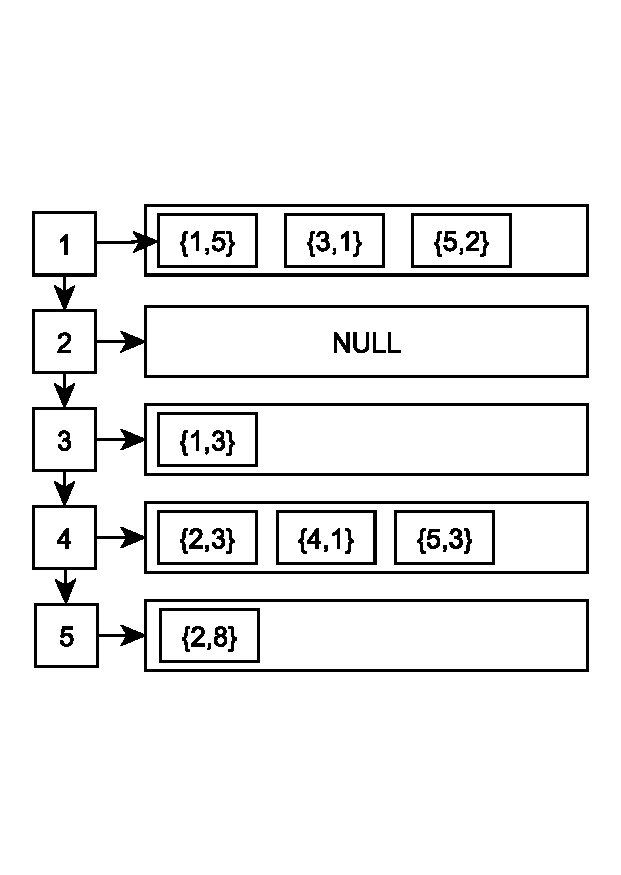
\includegraphics[width=0.5\textwidth, trim = 0mm 33mm 0mm 33mm, clip]{file_processing.pdf}
\caption{Struktura powstała po preprocessingu}
\label{fig:preprocessing_fig}
\end{figure}

Wynikiem działania tej części preprocesingu jest struktura będąca HashMapą, zawierająca komórce $i$ liste wszystkich niezerowych elementów znajdujących się w i-tym wierszu macierzy. Figura \ref{fig:preprocessing_fig} pokazuje fragment macierzy. Poniżej znajduje sie macierz $M_{5,5}$, która powstanie ze struktury przedstawionej na \ref{fig:preprocessing_fig}


\[
 M_{5,5} =
 \begin{pmatrix}
5 & 0 & 1 & 0 & 2\\
0 & 0 & 0 & 0 & 0\\
3 & 0 & 0 & 0 & 0\\
0 & 3 & 0 & 1 & 3\\
0 & 8 & 0 & 0 & 0\\

 \end{pmatrix}
\]


\section{Dane wyświetlane}
W tym kroku preprocessingu wyliczane są informacje przydatne przy wyświetlaniu wyników. Wyliczane jest kilka pierwszych najczęściej używanych tagów przy tych dokumentach i ilość użycia tych tagów w danym dokumencie. Dodatkowo zapisana jest informacja o ilości użytkowników którzy dany dokument dodali. Zapisywane są one w tabeli w formie tekstowej w bazie danych. W czasie wyświetlania wyników, dla wybranych dokumentów dane pobierane są z wyliczone wcześniej dane i przekazywane do wyświetlenia użytkownikowi. 


\section{Metody przyśpieszenia wykonywanych preprocesingów}

Jednym z głównym problemów jest to, że w czasie wykonywania wymienionych powyżej procedur, tabele USER, TAG i DOCUMENT są zablokowane na zmiany. W działającej aplikacji byłoby to poważnym problemem.  

Jedną z możliwości poradzenia sobie z tym problemem jest posiadanie kopi bazy danych i uzupełnianie obydwu jednocześnie. Dzięki czemu operacje wymagające dużej ilości czasu, mogłyby być wykonane na innej bazie. Po dokonaniu wszystkich obliczeń wymagane by było zsynchronizowanie dwóch baz danych.

Inną możliwością jest zrównoleglenie wykonywanych obliczeń. Możliwe jest na przykład: podzielenie obliczenia tabel TAG\_DOC, TAG\_USER i USERTAGDOC na różne maszyny. Dodatkową możliwością jest podzielenie samych tabel na różne procesy. Na przykład wyliczanie tabeli TAG\_DOC można podzielić na niezależne procesy ze względu na pole ID obiektów z tabeli TAG. Analogicznie można przeprowadzić taki podział dla innych tabel.

Inną możliwością są zmiany danych w tabelach TAG\_DOC, TAG\_USER i USERTAGDOC w czasie kiedy dodawane są nowe rekordy do tabel USER, DOCUMENT i TAG. Wyeliminowało by to potrzebę wykonywania opisane powyżej preprocesingu, ale stanowiło by problem przy tworzeniu macierzy. Tworzenie macierzy (dokładnie: plików z których następnie tworzona jest macierz) jest czasochłonne i wymaga zatrzymania zmian dokonywanych na tabelach TAG\_DOC, TAG\_USER i USERTAGDOC. Problem ten dałoby się rozwiązać przez np: posiadanie kopi wymienionych wcześniej tabel. Synchronizacja kopi tabeli i głównej tabeli nie zajmowała by aż tak wiele czasu. Pomysł ten spowodował by jeszcze jeden potencjalnie groźny problem. Ilość operacji, które trzeba by wykonać w czasie gdy dodawane są nowe rekordy do tabel, znacznie by się zwiększyła. Mogłoby to spowodować większą awaryjność np: problemy z transakcjami

\end{document}









